\documentclass[11pt,a4paper]{article}
\usepackage[T1]{fontenc}
\usepackage{lmodern}
\usepackage[margin=23mm]{geometry}
\usepackage{amsmath,amssymb,amsthm,microtype}
\usepackage{graphicx}
\usepackage{booktabs}
\usepackage[font={small,singlespacing}]{caption}
\usepackage{setspace}
\usepackage[hidelinks]{hyperref}
\setlength{\parindent}{0pt}
\setlength{\parskip}{6pt plus 1pt}
\setlength{\abovedisplayskip}{7pt plus 1pt}
\setlength{\belowdisplayskip}{7pt plus 1pt}
\newcommand{\tr}{\operatorname{tr}}
\newtheorem{theorem}{Theorem}
\newtheorem{lemma}{Lemma}
\newtheorem{proposition}{Proposition}
\begin{document}
\begin{center}
 {\Large\bfseries \textit{Keep Your Options Open}: Reducing Neurons Competition Through Overparameterization}
\end{center}

\section{Introduction}

A network can have enough parameters to represent a target and still struggle to find that representation. Why might adding width help, even when a narrower network is already expressive enough? We study one possibility: training that improves the current fit can change the network's ability to make a different correction later. Wider networks provide more possible implementations of a correction, and may retain useful responses when some implementations are altered by learning.

Such interactions can arise when the data contain shared structure as well as distinctions that matter only in particular contexts. Language provides a possible illustration: a common usage can account for much of the early error, while a less frequent context requires a different interpretation. Similarly, an image classifier may learn a broadly useful shape before learning a distinction that matters under an uncommon viewpoint. These are examples of the kind of imbalance we have in mind, not empirical claims about the experiments below. Frequency alone does not determine an update: residual size and parameter sensitivities matter too. Nevertheless, when many examples support a common correction, fitting it can dominate early training; a less frequent correction can then become important relative to the error that remains.

The two corrections need not have separate parameters. A hidden unit that helps fit the common pattern may also contribute to a contextual distinction. Moving it to improve the former can strengthen, weaken, or remove its response to the latter. We call a decrease in the capability needed for one correction, caused by an update driven by another, \emph{competition}. This is a statement about how learning changes the available response, not merely about two examples having different labels.

Our central object is an \emph{option}: a correction demanded by the residual together with the network's ability to make it. Imagine that two contexts still require different predictions but the network's parameters currently affect them in nearly the same way. The distinction is needed, yet the corresponding option is weak. If the response disappears entirely while the distinction is still needed, the option is closed at that state. By contrast, if the model has already fitted the distinction, the demand has disappeared; this is not a lost option. The difference matters because weak responses can recover, and alternative implementations can preserve a correction even when one unit stops contributing.

We first derive these ideas from prediction dynamics and define a measurable response at a checkpoint. We then study a shallow ReLU network in which dominant learning changes exposed units but leaves some alternatives protected. A completion-reserve curve uses this mechanism to predict response after a specified amount of learning. Finally, controlled co-occurrence and parity experiments test the prediction and its limits. The aim is to explain when width can preserve needed corrections and, ultimately, when this preservation matters for loss.

\section{Options and competition}
\label{sec:core}

\subsection{From parameter updates to prediction dynamics}

Let $\mathcal D=\{(x_i,y_i)\}_{i=1}^n$ be a dataset, $\theta\in\mathbb R^P$ the parameters, and $F(\theta)=(f_\theta(x_i))_{i=1}^n$ the predictions. Write $e=y-F(\theta)$ for the residual and take squared loss $L(\theta)=\|e\|^2/(2n)$. The prediction Jacobian $J_\theta\in\mathbb R^{n\times P}$ has row $i$ equal to $\nabla_\theta f_\theta(x_i)^T$. For a small parameter change, $F(\theta+\delta\theta)-F(\theta)\simeq J_\theta\delta\theta$: each column of $J_\theta$ is a pattern of prediction changes available through one parameter.

The loss gradient is $\nabla_\theta L=-J_\theta^Te/n$. In the continuous-time limit of full-batch gradient descent, the chain rule therefore gives
\begin{equation}
 \dot\theta=\frac1n J_\theta^T e,\qquad
 \dot e=-K_\theta e,\qquad K_\theta=\frac1nJ_\theta J_\theta^T.
 \label{eq:flow}
\end{equation}
The two appearances of the Jacobian have distinct roles: $J_\theta^T$ turns residuals into parameter motion, and $J_\theta$ turns that motion into prediction changes. The entry $(K_\theta)_{ij}$ describes how residual on example $j$ contributes to the prediction velocity on example $i$. In particular, the predictions of two inputs are coupled when their parameter sensitivities have a nonzero inner product.

The kernel is positive semidefinite because $d^TK_\theta d=\|J_\theta^Td\|^2/n\ge0$ for every prediction-space direction $d$. Consequently $\dot L=-e^TK_\theta e/n\le0$ under this flow. Equation~\eqref{eq:flow} describes the actual nonlinear network instantaneously: the Jacobian and kernel generally change as training moves the parameters. At ReLU boundaries the derivatives require a piecewise convention, and a finite gradient step need not obey the continuous equation exactly.

\subsection{What can the current network correct?}

To describe the capability present at an actual checkpoint $s$, let $\theta_s=\theta(s)$, $e_s=y-F(\theta_s)$, and $J_s=J_{\theta_s}$. We temporarily freeze the derivatives and study the first-order model
\begin{equation}
 \widehat f_s(\delta\theta,x)=f_{\theta_s}(x)+\nabla_\theta f_{\theta_s}(x)^T\delta\theta.
 \label{eq:linearization}
\end{equation}
This model is linear in the parameter displacement $\delta\theta$, though it can of course be nonlinear in $x$. It tells us how much error could be removed if the sensitivities observed at checkpoint $s$ stayed fixed?

Let $t$ denote time in this auxiliary model, with $\delta\theta=0$ initially. Its constant kernel is $K_s=J_sJ_s^T/n$. Equation~\eqref{eq:flow} becomes $d\widehat e_s/dt=-K_s\widehat e_s$, so $\widehat e_s(t)=e^{-tK_s}e_s$. To see what this means, let $K_sv_i=\kappa_i v_i$ for orthonormal eigenvectors $v_i$ and nonnegative eigenvalues $\kappa_i$. The residual component along $v_i$ evolves as
\begin{equation}
 v_i^T\widehat e_s(t)=e^{-t\kappa_i}v_i^Te_s.
 \label{eq:modal-decay}
\end{equation}
Each $v_i$ is a pattern of prediction error and $\kappa_i$ is its local correction rate. A zero rate means that the frozen model cannot reduce that component. For example, if two examples have identical prediction gradients, every first-order parameter change affects their predictions equally; their difference is a zero-rate direction. The nonlinear network might later acquire a response to it as its parameters move.

For $\widehat L_s(t)=\|\widehat e_s(t)\|^2/(2n)$, the local loss reduction is
\begin{equation}
 \widehat L_s(0)-\widehat L_s(t)
 =\frac{1}{2n}e_s^T B_{s,t}e_s,\qquad
 B_{s,t}=I-e^{-2tK_s}.
 \label{eq:benefit}
\end{equation}
The response strength of mode $i$ is $\beta_i(t)=1-e^{-2t\kappa_i}$: if all the initial residual lies in that mode, this is the fraction of its loss removed by time $t$. A positive rate can be too slow to make much progress within the available time. For example, at $t=1$, rates $10$ and $0.01$ remove nearly all and about $2\%$ of their respective modal losses.

\subsection{Combining response and demand through options}

A fast correction is useful only if it is needed. Let $E$ be an eigenspace of $K_s$, $\Pi_E$ its orthogonal projector, and $q_E=\Pi_Ee_s$ the residual component in that space. When $q_E\ne0$, we call the demanded correction $q_E$ together with its response an \emph{option}. Its value over horizon $t$ is
\begin{equation}
 v_{s,t}(E)=\frac{1}{2n}\,\beta_E(t)\|q_E\|^2,
 \qquad \beta_E(t)=1-e^{-2t\kappa_E}.
 \label{eq:option-value}
\end{equation}
The two factors have different meanings: $\|q_E\|^2/(2n)$ is the initial loss associated with the demand, while $\beta_E(t)$ is the fraction the local model can remove. Summing the option values over eigenspaces recovers equation~\eqref{eq:benefit}.

An option is \emph{open} when its demand is nonzero and its correction rate is positive; it is \emph{closed} when demand is nonzero but the rate is zero. A very weak open option may still have little value within the horizon. If $q_E=0$, there is no current demand in that eigenspace, regardless of its rate. This distinction is essential when comparing checkpoints: a falling residual can mean the task has been learned, whereas a falling response to the same fixed correction can indicate a lost capability.

For a summary over several horizons, average $B_{s,t}$ with density $\tau^{-1}e^{-t/\tau}$, whose mean is $\tau$. The resulting \emph{discounted response operator} is
\begin{equation}
 C_{s,\tau}=\int_0^\infty\frac{e^{-t/\tau}}{\tau}B_{s,t}\,dt
 =K_s(K_s+\lambda I)^{-1},\qquad \lambda=(2\tau)^{-1}.
 \label{eq:response}
\end{equation}
On a mode with rate $\kappa$, the average strength is $\bar\beta=\kappa/(\kappa+\lambda)$, and its discounted option value is $\bar\beta\|q_E\|^2/(2n)$. Thus $e_s^TC_{s,\tau}e_s/(2n)$ is the average frozen-model loss reduction. The scale $\tau$ selects what counts as a useful speed; it is part of the measurement, not a change to the training objective or an assumed stopping time.

We can also measure capability without requiring a particular current residual. For a fixed unit vector $d$ in prediction space, define $\beta(d)=d^TC_{s,\tau}d$. For example, $d$ can represent the difference between predictions on two contexts that we want to distinguish. We call it a \emph{probe}: it specifies the correction whose response we want to inspect.

\subsection{How one correction can weaken another}

Suppose that the residual is decomposed as $e=p+r$: for example, $p$ contains errors on common-context examples and is zero elsewhere, while $r$ contains errors on the remaining examples. Equation~\eqref{eq:flow} gives the exact decomposition $\dot\theta=J_\theta^Tp/n+J_\theta^Tr/n$. Both terms use the original dataset weighting, so a smaller subset is not artificially renormalized to have the same influence as a larger one. We call the two contributions \emph{pressures} because each describes how a set of residuals drives the shared parameters.

To isolate what learning $p$ does to the capability needed for $r$, hold $r$ fixed and differentiate the response along $\dot\theta_p=J_\theta^Tp/n$. Suppress the checkpoint subscript and write $R=(K+\lambda I)^{-1}$. Since $C_\tau=I-\lambda R$, differentiating the inverse yields $\dot C_\tau[p]=\lambda R\dot K[p]R$, where $\dot K[p]$ is the kernel's derivative along the $p$-driven velocity. We define the local competition score as
\begin{equation}
 \mathfrak C_\tau(p\!\to\!r)=-\frac{1}{2n}r^T\dot C_\tau[p]r.
 \label{eq:competition}
\end{equation}
A positive score means that the $p$-driven update weakens the response available to the fixed correction $r$; a negative score means it strengthens that response. The fixed reference is important: if we also differentiated $r$, a reduction in demand from successful fitting could be mistaken for weakening. At a ReLU crossing, the derivative may not exist. Local weakening does not by itself prove a lasting penalty. The weakened response must overlap demand that remains or arises later, and other implementations or recovery must fail to compensate within the training budget.

\section{Protected reserve and completion of dominant learning}
\label{sec:reserve}

Section~\ref{sec:core} measures which corrections a network can make at a given state. We now ask how that capability changes as the network learns a dominant part of the task.

\subsection{What can dominant learning leave untouched?}

Consider the shallow ReLU network
\begin{equation}
 f_\theta(x)=c+\frac1m\sum_{j=1}^m a_j[w_j^Tx]_+,
 \qquad [z]_+=\max(z,0),
 \label{eq:network}
\end{equation}
where $w_j$ and $a_j$ are the incoming weights and readout coefficient of unit $j$, and $c$ is an output intercept. Let the data distribution assign probability $p_k$ to input $x_k$ and target $y_k$, and write $e_k=y_k-f_\theta(x_k)$. For squared loss $L=\frac12\sum_k p_ke_k^2$, we use the update scaling of the experiments: the incoming and readout velocities are $m$ times their ordinary negative gradients, while the intercept uses the ordinary gradient. The resulting dynamics are
\begin{equation}
 \dot c=\sum_k p_ke_k,\qquad
 \dot a_j=\sum_k p_ke_k[w_j^Tx_k]_+,\qquad
 \dot w_j=a_j\sum_k p_ke_k\mathbf1_{w_j^Tx_k>0}x_k.
 \label{eq:weighted-dynamics}
\end{equation}
The last two equations show the coupling that matters here: the unit's activation drives its readout, and its readout scales the motion of its incoming weights. In particular, if $w_j^Tx_k<0$, that example produces no update to either part of the unit.

As in Section~\ref{sec:core}, the kernel combines parameter sensitivities into a measure of response in prediction space. For this weighted loss and update scaling, let $D_p=\operatorname{diag}(p_1,\ldots,p_n)$, let $J$ be the prediction Jacobian, and let $M=\operatorname{diag}(mI,\ldots,mI,1)$ contain the update multipliers. The resulting kernel is
\begin{equation}
 K=D_p^{1/2}J M J^T D_p^{1/2}
   =bb^T+\frac1m\sum_{j=1}^m Z_j,
 \qquad b_k=\sqrt{p_k}.
 \label{eq:weighted-kernel}
\end{equation}
Here $bb^T$ is the intercept's contribution and each $Z_j\succeq0$ is the sensitivity contribution of unit $j$, including both $w_j$ and $a_j$. The weighted residual is $D_p^{1/2}e$, and the discounted response operator remains $C_\tau(K)=K(K+\lambda I)^{-1}$, with $\lambda=(2\tau)^{-1}$. The important feature of the decomposition is that every unit adds a positive semidefinite contribution: removing some units from the sum cannot increase the kernel.

Suppose a dominant component of training uses inputs in a set $\mathcal H$. A unit is \emph{protected} against this component if it is inactive on all of $\mathcal H$: $w_j^Tx<0$ for every $x\in\mathcal H$. Even if it responds to other inputs, equation~\eqref{eq:weighted-dynamics} shows that dominant-only updates do not change its parameters. Let $\mathcal F_{\mathcal H}$ be the units protected at a chosen starting state. Their initial contribution, together with the intercept, defines the \emph{protected kernel}
\begin{equation}
 K_{\mathcal H}^{\rm safe}=bb^T+\frac1m\sum_{j\in\mathcal F_{\mathcal H}}Z_j(0).
 \label{eq:safe}
\end{equation}
The denominator remains $m$: this is the protected contribution within the original network, not a smaller network rescaled to have the same total weight.

\begin{theorem}[Protected reserve]\label{thm:reserve}
Fix the data distribution and the units initially protected against $\mathcal H$. For gradient flow or discrete gradient updates driven only by inputs in $\mathcal H$,
\begin{equation}
 K(t)\succeq K_{\mathcal H}^{\rm safe},\qquad
 C_\tau(K(t))\succeq C_\tau(K_{\mathcal H}^{\rm safe}).
 \label{eq:reserve-bound}
\end{equation}
The inequalities hold for any sequence of such updates, irrespective of the sign of their residuals.
\end{theorem}

The reason is simple: the protected units stay fixed, the intercept's sensitivity is constant, and all other units contribute positive semidefinite terms. The same ordering carries over to $C_\tau$. Consequently, for any fixed correction direction $d$, the quantity $\beta^{\rm safe}(d)=d^TC_\tau(K_{\mathcal H}^{\rm safe})d$ is a lower bound on its response after any amount of dominant-only learning. This is the \emph{protected reserve} for that correction. Two networks can have similar current response $\beta(d)=d^TC_\tau(K)d$ yet different reserves: one may rely mostly on units exposed to dominant updates, while the other retains response through units those updates cannot move.

The guarantee concerns capability, not whether the correction is currently demanded or whether the model will fit it. It also depends on the source of the updates. Examples outside $\mathcal H$ can move the initially protected units, so the original floor need not survive full training. Its practical value depends on whether their cumulative effect is small, but a low occurrence probability alone does not establish that. The floor can also be zero, for example if no protected unit supports the correction. In that case it says nothing about the response retained by exposed units, which motivates the next calculation.

\subsection{Predicting response after a learning phase}

To predict what happens to exposed units, we need to identify the pressure driving the phase. In the controlled bridge experiment of Section~\ref{sec:results}, the dominant input is known. More generally, we can look for a direction directly in the incoming-weight updates. Form the matrix $G_W$ whose $j$th row is $\dot w_j^T$, and take its singular value decomposition $G_W=\sum_i\sigma_i u_i v_i^T$. The leading right singular vector $\hat u=v_1$ is the direction along which the units have the largest total squared incoming motion. The ratio $\rho=\sigma_1^2/\sum_i\sigma_i^2$ measures the fraction of that motion captured by the direction.

This provides a candidate axis from the observed gradient without a label for the dominant factor. Its sign can be oriented using the residual pressure. A high $\rho$ makes a one-direction description plausible at that checkpoint, but does not guarantee that the direction remains stable, that readout weights follow the required dynamics, or that other updates are negligible. The parity experiment tests both the estimated direction and the resulting response prediction.

We therefore start with an idealized phase driven only by one input $u$ and derive what such a phase would do. Take $\|u\|=1$ and suppose its residual is positive. The same calculation extends to inputs of other lengths by retaining their scale; the parity forecast estimates a scale along the detected direction. For unit $j$, write $W_j=w_j^Tu$ for the incoming weight along $u$ and $A_j=a_j$ for the readout. Let $s(t)=\int_0^t p_{\rm dom}e_{\rm dom}(v)\,dv$ be the cumulative pressure from this input; it measures how much of the dominant update has been applied. While the unit is active on $u$, equation~\eqref{eq:weighted-dynamics} gives $dW_j/ds=A_j$, $dA_j/ds=W_j$, and $dc/ds=1$. Thus
\begin{equation}
 W_j(s)=W_j(0)\cosh s+A_j(0)\sinh s,\qquad
 A_j(s)=A_j(0)\cosh s+W_j(0)\sinh s.
 \label{eq:hyperbolic}
\end{equation}
The component of $w_j$ perpendicular to $u$ stays fixed. If $W_j$ reaches zero, the unit becomes inactive on $u$ and stops moving under this pressure; an initially inactive unit stays fixed from the start. Equation~\eqref{eq:hyperbolic} therefore applies only while the dominant gate is active. We denote the full state obtained by following these dynamics and stopping units at their gates by $\Phi_s(\theta)$.

This motion can affect an input other than $u$. For example, a unit with $W_j>0$ and $A_j>0$ moves further in the $u$ direction. If another input points partly opposite to $u$, its preactivation in that unit can decrease and its gate can close. A different unit may remain active there, preserving the distinction. The state transformation $\Phi_s$ keeps track of all units together, including protected ones, so the resulting response need not decline simply because one gate closes. Appendix~\ref{app:flow} works out the closure condition for a symmetric pair of inputs.

The amount of pressure $s$ is not yet the quantity we want to specify: the phase is more naturally described by what the network has learned. Let $F(s)=f_{\Phi_s(\theta)}(u)$ be the prediction on the dominant input. Between gate events,
\begin{equation}
 F'(s)=1+\frac1m\sum_{j:W_j(s)>0}\bigl(W_j(s)^2+A_j(s)^2\bigr)>0.
 \label{eq:gain}
\end{equation}
The first term comes from the output intercept. The prediction is continuous at gate events, so $F$ is strictly increasing throughout the idealized flow. For any desired gain $C\ge0$, there is therefore a unique exposure $s_C$ satisfying $F(s_C)-F(0)=C$.

Now fix a correction direction $d_r$ and evaluate its response at that state. The resulting \emph{completion-reserve curve} is
\begin{equation}
 \mathcal R_r(C;\theta)=d_r^TC_\tau\!\left(K(\Phi_{s_C}(\theta))\right)d_r.
 \label{eq:completion}
\end{equation}
At $C=0$ this is the current response. At a positive $C$, it answers: \emph{if the network makes this much progress on the dominant input under the idealized flow, how much response to the other correction remains?} It adds a finite-phase prediction to the protected floor by accounting for the exposed units as well.

This is the quantity tested in Section~\ref{sec:results}. At the start of each phase we specify a dominant prediction gain and compute $\mathcal R_r$ for each correction. A predicted half-response loss occurs when $\mathcal R_r(C;\theta)<\tfrac12\mathcal R_r(0;\theta)$; the observed event uses the actual response at the end of full training for that phase.

\section{Empirical evaluation}
\label{sec:results}

\subsection{Tasks and measurements}

We use three related synthetic tasks to examine the mechanism at different levels. A \emph{three-pattern task} has one frequent input and two rare inputs with opposite targets. It makes a single needed distinction easy to follow, so we can compare response and loss during training. A \emph{co-occurring-factor task} extends this setting to four rare signed factors, several of which can occur in the same example. Its frequencies and overlap can be varied to test the model over many initializations. Both tasks have an exact three-unit representation, so the narrower networks considered below can represent their targets.

The \emph{parity task} instead has unequal-frequency binary factors $B_i$ and target $y=(-1)^{\sum_i B_i}$. Its standardized inputs and bipolar targets produce a frequent, initially unlearned pattern and opposing input directions. This task tests whether a useful dominant direction can be estimated from the gradient, and whether the resulting response prediction transfers to a target defined by interactions among factors.

All experiments train the full network on the full squared-loss objective. To compare response before and after a phase, we follow fixed factor contrasts rather than changing kernel eigenvectors. For comparability, these response measurements weight the tested contrasts equally rather than by their population frequencies; loss is evaluated using the data distribution. A contrast measures capability and is not automatically a spectral option. Its loss of response is consequential only when demand remains.

\subsection{From a lost response to loss}

Figure~\ref{fig:learning} illustrates the proposed chain in the three-pattern task. The narrow network loses its response to the rare distinction while the wider network retains it. The reserve calculation predicts the narrow closure from the initial state, and the observed closure occurs nearby. This happens while the common pattern still dominates the loss: the learning curves separate only later, when the rare distinction matters more. The narrow network then remains near a loss floor, while the wider one continues improving.

The dotted floor is a \emph{conditional} loss prediction. In this example, the additional gate conditions trap the narrow network with the same prediction on the two rare inputs; because their targets are opposite, a residual loss remains even after the best shared prediction. The predicted floor follows from those conditions, not from a low response alone. The full loss curves are observed, not forecast by completion reserve. This width pair was selected using its initial state before training outcomes were computed, so it illustrates the mechanism rather than estimating how often it occurs or proving that width caused the loss gap.

\begin{figure}[htbp]
\centering
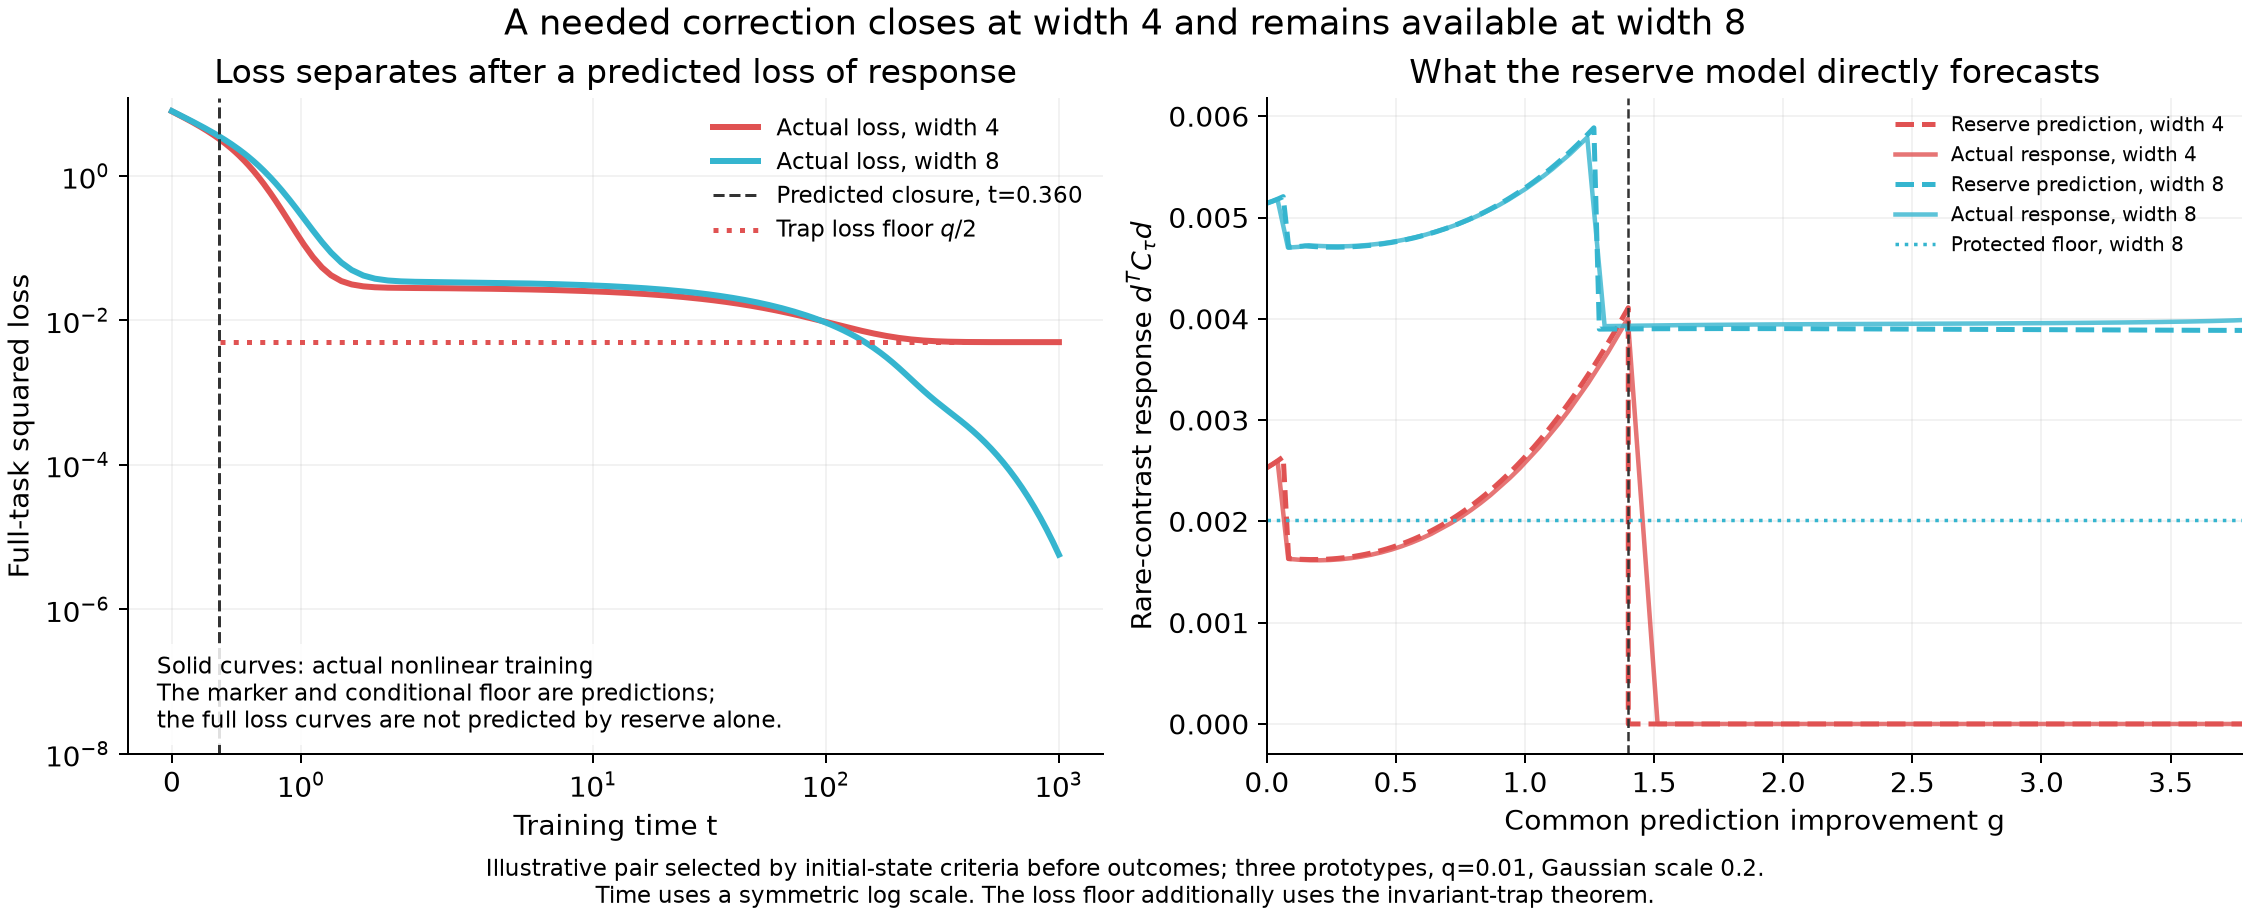
\includegraphics[width=0.86\linewidth]{figures/learning_and_reserve.png}
\caption{Selected three-pattern example: observed loss and response at widths 4 and 8, with reserve-based response predictions. The loss floor additionally uses the conditional gate-trap argument.}
\label{fig:learning}
\end{figure}

\subsection{How often is response weakened?}

The example motivates an aggregate question: how likely is substantial weakening during a learning phase, and does width change it? We define a half-response loss as a response falling below half its starting value by the time the dominant prediction has corrected half its remaining error. At the start of each phase, the completion-reserve curve predicts whether that event will occur; the network is then trained on all examples, including the rare ones.

Table~\ref{tab:bridge} compares the resulting predicted and observed event frequencies for independently co-occurring factors. Each frequency estimates the chance of an event for a factor and phase drawn from the stated experiment; the model's frequency is the fraction of its deterministic phase predictions, not a calibrated probability assigned to each correction. Initializations are independent, but factors and phases within an initialization are not. The model reproduces the strong reduction in weakening with width and ranks vulnerable corrections better than current response alone. This supports the idea that the response left after dominant learning matters more than current response in this setting. The near absence of events at the largest width makes its ranking score uncertain.

\begin{table}[htbp]
\centering
\caption{Predicted and observed half-response loss frequencies for independently co-occurring factors ($Q=0.04$), with 1,024 factor--phase observations from 128 initializations per width. AUC measures event ranking; 0.5 is chance.}
\label{tab:bridge}
\begin{tabular}{@{}lrrrr@{}}
\toprule
Width & Predicted & Observed & Completion AUC & Current-response AUC \\
\midrule
4  & 6.35\% & 6.64\% & 0.988 & 0.577 \\
8  & 1.66\% & 1.76\% & 0.944 & 0.692 \\
16 & 0.10\% & 0.20\% & 0.991 & 0.510 \\
\bottomrule
\end{tabular}
\end{table}

The unchanged predictor also transfers to a distribution with much more factor overlap. Its accuracy deteriorates, however, when updates from the other factors become a larger part of training. This is the expected limitation of approximating full training by a single dominant pressure: co-occurrence need not invalidate the mechanism, but the additional updates cannot always be neglected. The selected example above and these event frequencies answer different questions; neither establishes that the aggregate reduction in weakening causes an aggregate loss advantage.

\subsection{A harder test: parity}

On parity, the leading gradient direction aligns increasingly well with the known dominant direction as width grows, and the updates are reasonably concentrated along it (Table~\ref{tab:parity}). Nevertheless, the completion model misses most of the half-response losses observed in the narrow network. The same undercount occurs when the known direction is supplied, so direction estimation alone does not explain the error. Wider networks have fewer observed weakening events and lower final loss in this sample, but zero observed events do not prove immunity, and the loss comparison does not establish that response weakening caused the difference.

\begin{table}[htbp]
\centering
\caption{Four-factor parity: half-response losses, gradient-direction coherence and alignment, and mean population loss at the final checkpoint. Each width has 512 tested contrasts.}
\label{tab:parity}
\begin{tabular}{@{}lrrrrr@{}}
\toprule
Width & Observed & Predicted & Coherence & Alignment & Final loss \\
\midrule
4  & 8 & 1 & 0.830 & 0.738 & 0.0826 \\
8  & 0 & 0 & 0.759 & 0.818 & 0.0712 \\
16 & 0 & 0 & 0.728 & 0.890 & 0.0607 \\
32 & 0 & 0 & 0.716 & 0.935 & 0.0520 \\
\bottomrule
\end{tabular}
\end{table}

Together, these results show how reserve can connect an individual loss of response to later loss, and when it can predict aggregate weakening. They also show the next question: whether weakened responses persist while demand remains, or recover before they materially affect loss. Parity demonstrates that a coherent direction is not by itself sufficient for the current completion approximation.

\clearpage
\appendix
\section{Proof of the protected-reserve result}\label{app:reserve}
Let $P=K_{\mathcal H}^{\rm safe}$ and let $K(t)$ be evaluated on the fixed data distribution. Initially protected units have zero activation and zero incoming and readout gradients on the pressure support. With the stated update rule they remain fixed by induction for discrete steps, and the same argument applies along gradient flow. The intercept derivative block is constant. Therefore $K(t)-P$ is a sum of the other units' positive semidefinite Gram blocks, so $K(t)\succeq P$.

For positive definite matrices, inversion reverses the Loewner order. Thus $(K(t)+\lambda I)^{-1}\preceq(P+\lambda I)^{-1}$, and $C_\tau(K)=I-\lambda(K+\lambda I)^{-1}$ gives the response inequality. This proves Theorem~\ref{thm:reserve}; it applies to any fixed probe or residual by taking the corresponding quadratic form.

Under full training, let $P_t$ be the kernel of the originally protected blocks at time $t$, together with the constant intercept block. For a unit correction $d$, the corresponding response satisfies
\begin{equation}
 \beta_t(d)\ge d^TC_\tau(P)d-\frac{\|P_t-P\|_{\rm op}}{\lambda}.
 \label{eq:perturb}
\end{equation}

The remaining blocks are positive semidefinite, hence $C_\tau(K(t))\succeq C_\tau(P_t)$. The resolvent identity gives
\[
 C_\tau(P_t)-C_\tau(P)
 =\lambda(P_t+\lambda I)^{-1}(P_t-P)(P+\lambda I)^{-1}.
\]
Both inverse norms are at most $1/\lambda$. For a unit probe, the absolute quadratic-form difference is consequently at most $\|P_t-P\|_{\rm op}/\lambda$, proving equation~\eqref{eq:perturb}. No small-drift claim follows without an additional bound on $P_t-P$.

\section{Transport, gate stopping, and closure}\label{app:flow}
For the common-only input $u$ and squared loss, write $s(t)=\int_0^t p_{\rm dom}e_{\rm dom}(v)\,dv$. In a phase with positive pressure, an active unit obeys $dW/ds=A$ and $dA/ds=W$; its perpendicular weight is constant and $dc/ds=1$. The equations yield $d(W+A)/ds=W+A$ and $d(W-A)/ds=-(W-A)$, which give equation~\eqref{eq:hyperbolic}. They also preserve $A^2-W^2$. The active solution reaches zero at finite positive exposure exactly when $A<-W$; at the hit, both incoming and readout gradients from $u$ vanish under the zero-at-zero convention. The stopped solution therefore remains at the boundary for the rest of this common-only phase.

For an example of how dominant learning can close a different correction, consider two equally probable inputs $x_{r\pm}=-\cos\vartheta\,u\pm\sin\vartheta\,v_r$, where $u$ and $v_r$ are orthogonal unit vectors and $0<\vartheta<\pi/2$. Assume strictly positive readout coefficients and consider the contrast between the pair. The unit's preactivations are $-\cos\vartheta\,W\pm\sin\vartheta\,B$, with $B=w^Tv_r$ constant. Both are nonpositive exactly when $W\ge\tan\vartheta|B|=T$. For $W>0$, $A>0$, $W(s)$ increases strictly. Solving $W\cosh s+A\sinh s=T$ for $e^s$ gives the closing exposure
\begin{equation}
 s_{jr}=\log\!\left(\frac{T+\sqrt{T^2+A^2-W^2}}{W+A}\right)
 \label{eq:closing}
\end{equation}
when $T>W$; if $T\le W$ the unit is already blind. A common-inactive unit is fixed and, when it supports the contrast, remains a route indefinitely.

The kernel is a sum of derivative Gram blocks. With positive readouts, an open gate on either member of the symmetric pair contributes a nonzero derivative in the antisymmetric contrast direction; with both gates closed the contribution is zero. Hence the contrast is in the kernel nullspace if and only if every unit contribution is zero. Since each common-active unit's rare gates close monotonically in this sector, the last such event is $s_r^*=\max_j s_{jr}$. If any protected route remains, this maximum is infinite. The resolvent has the same nullspace as the positive semidefinite kernel, so this is also exact zero discounted response.

\end{document}
